\documentclass[
	A4paper,
	DIV=9,
	BCOR7mm,
	smallheadings,
	headinclude,
	footinclude,
	headsepline,
	parindent,
	german,
	captions=tableheading,
	abstracton
	]{scrreprt}
\usepackage{blindtext}
\usepackage[ngerman]{babel}
\usepackage[T1]{fontenc}
\usepackage[utf8]{inputenc}
\usepackage{lmodern}
\usepackage{microtype}
\usepackage{geometry}
\usepackage{graphicx}
\usepackage{amssymb}
\usepackage{xcolor}
\usepackage{hyperref}
\hypersetup{
		colorlinks	= true,
		linkcolor	= blue,
		urlcolor	= blue,
		citecolor	= blue,
		pdftitle    = {},
  		pdfsubject  = {},
  		pdfauthor   = {Panagiota Sismanidou},
  		pdfkeywords = {} ,
  		pdfcreator  = {pdflatex},
  		pdfproducer = {LaTeX with hyperref}
	}
\usepackage[style=apa]{biblatex}
\bibliography{Literaturverzeichnis}


\title{Enterprise Architecture Management}
\author{Panagiota Sismanidou}
\date{30.08.2018}

\begin{document}
\maketitle

\tableofcontents

\chapter{Theorie}
\section{Unterpunkt 1}
\chapter{Fallstudien}
\section{Unterpunkt 1}


\blindtext[1]{}\autocite{:Geschwinde_Rauschdrogen}

\blindtext[2]{}\blindtext[1]{}\autocite{:Muelhardt_2013}
\begin{figure}[htbp]
\begin{center}
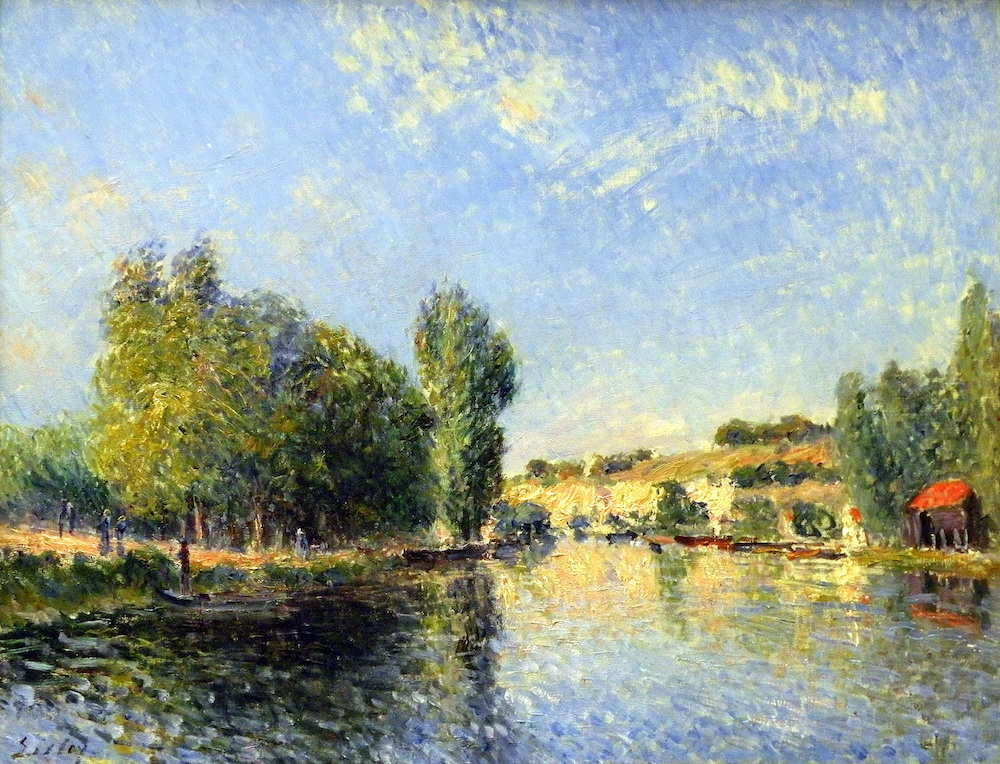
\includegraphics[width=0.7\textwidth]{Abbildungen/Bild1.jpg}
\caption{Bild 1}
\label{fig:Bild1}
\end{center}
\end{figure}

\blindtext[2]{}\autocite{:Wintermantel_Medizintechnik}
\begin{figure}[htbp]
\begin{center}
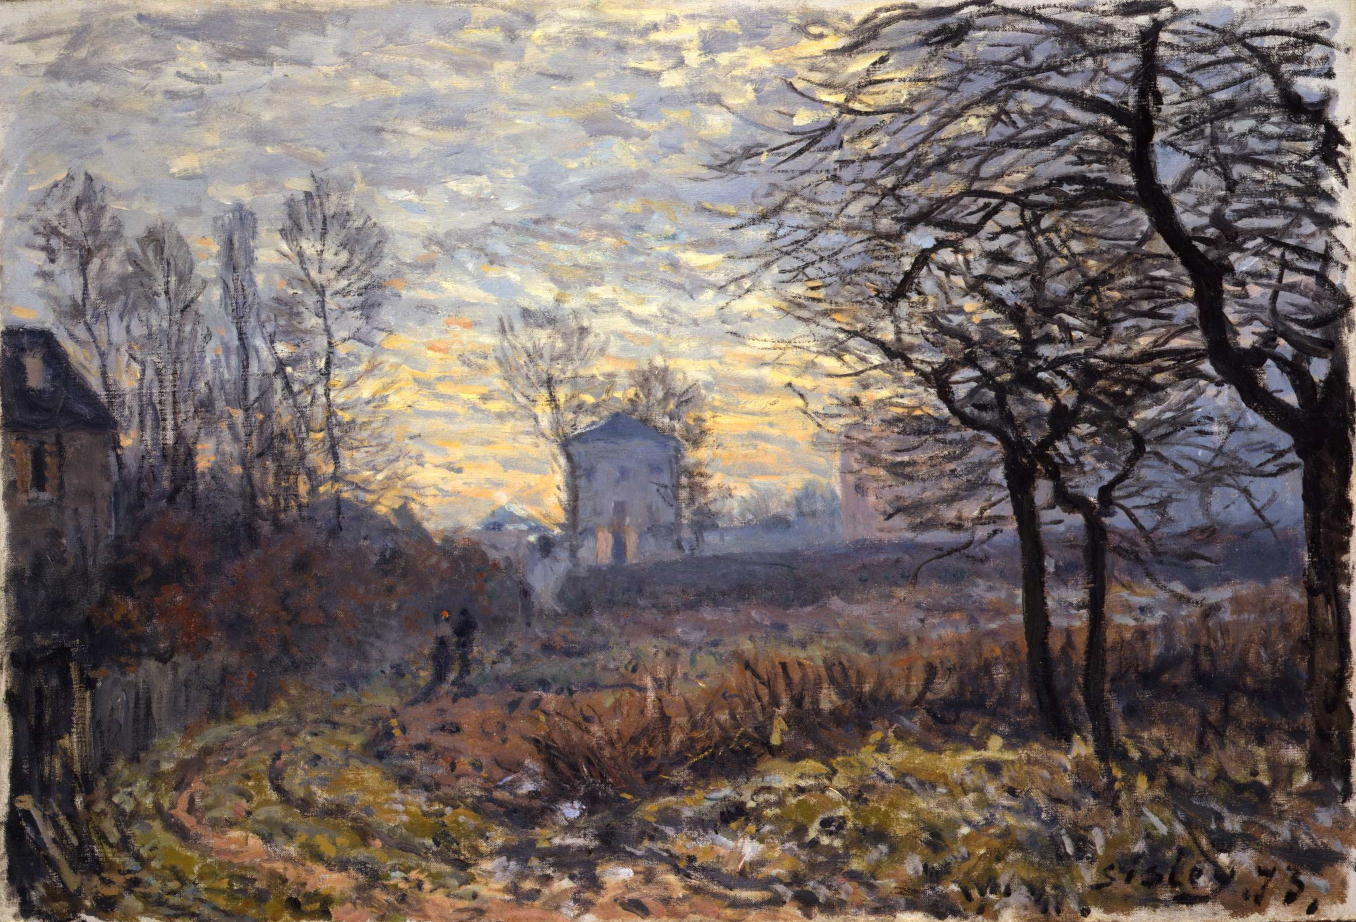
\includegraphics[width=0.7\textwidth]{Abbildungen/Bild2.jpg}
\caption{Bild 2}
\label{fig:Bild2}
\end{center}
\end{figure}

\blindtext[1]{}\autocite{:Keshk_2014}
\section{Unterpunkt 2}
\blindtext[1]{}\autocite{:Aydin_2009}

\blindtext[1]{}\autoref{fig:Bild3}
\blindtext[1]{}\autocite{:Muelhardt_2013}
\begin{figure}[htbp]
\begin{center}
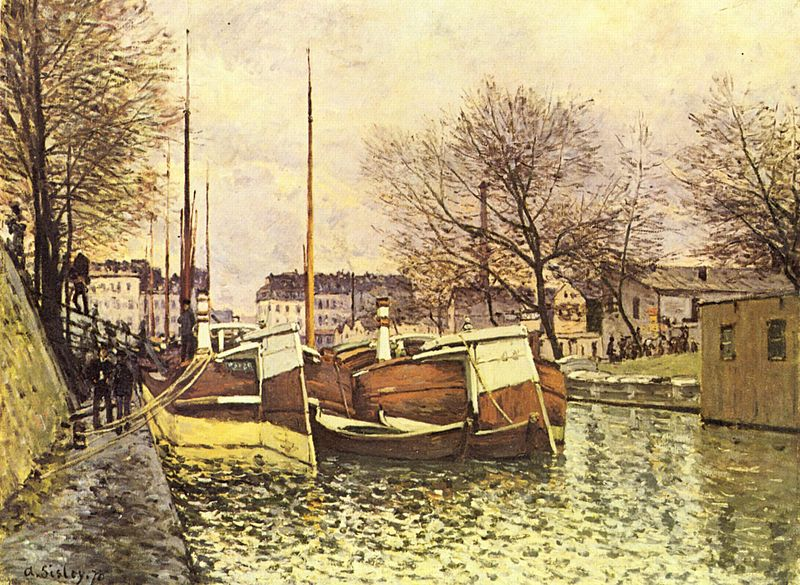
\includegraphics[width=0.7\textwidth]{Abbildungen/Bild3.jpg}
\caption{Bild 3}
\label{fig:Bild3}
\end{center}
\end{figure}

\blindtext[2]{}\autocite{:Geschwinde_Rauschdrogen}
\begin{figure}[htbp]
\begin{center}
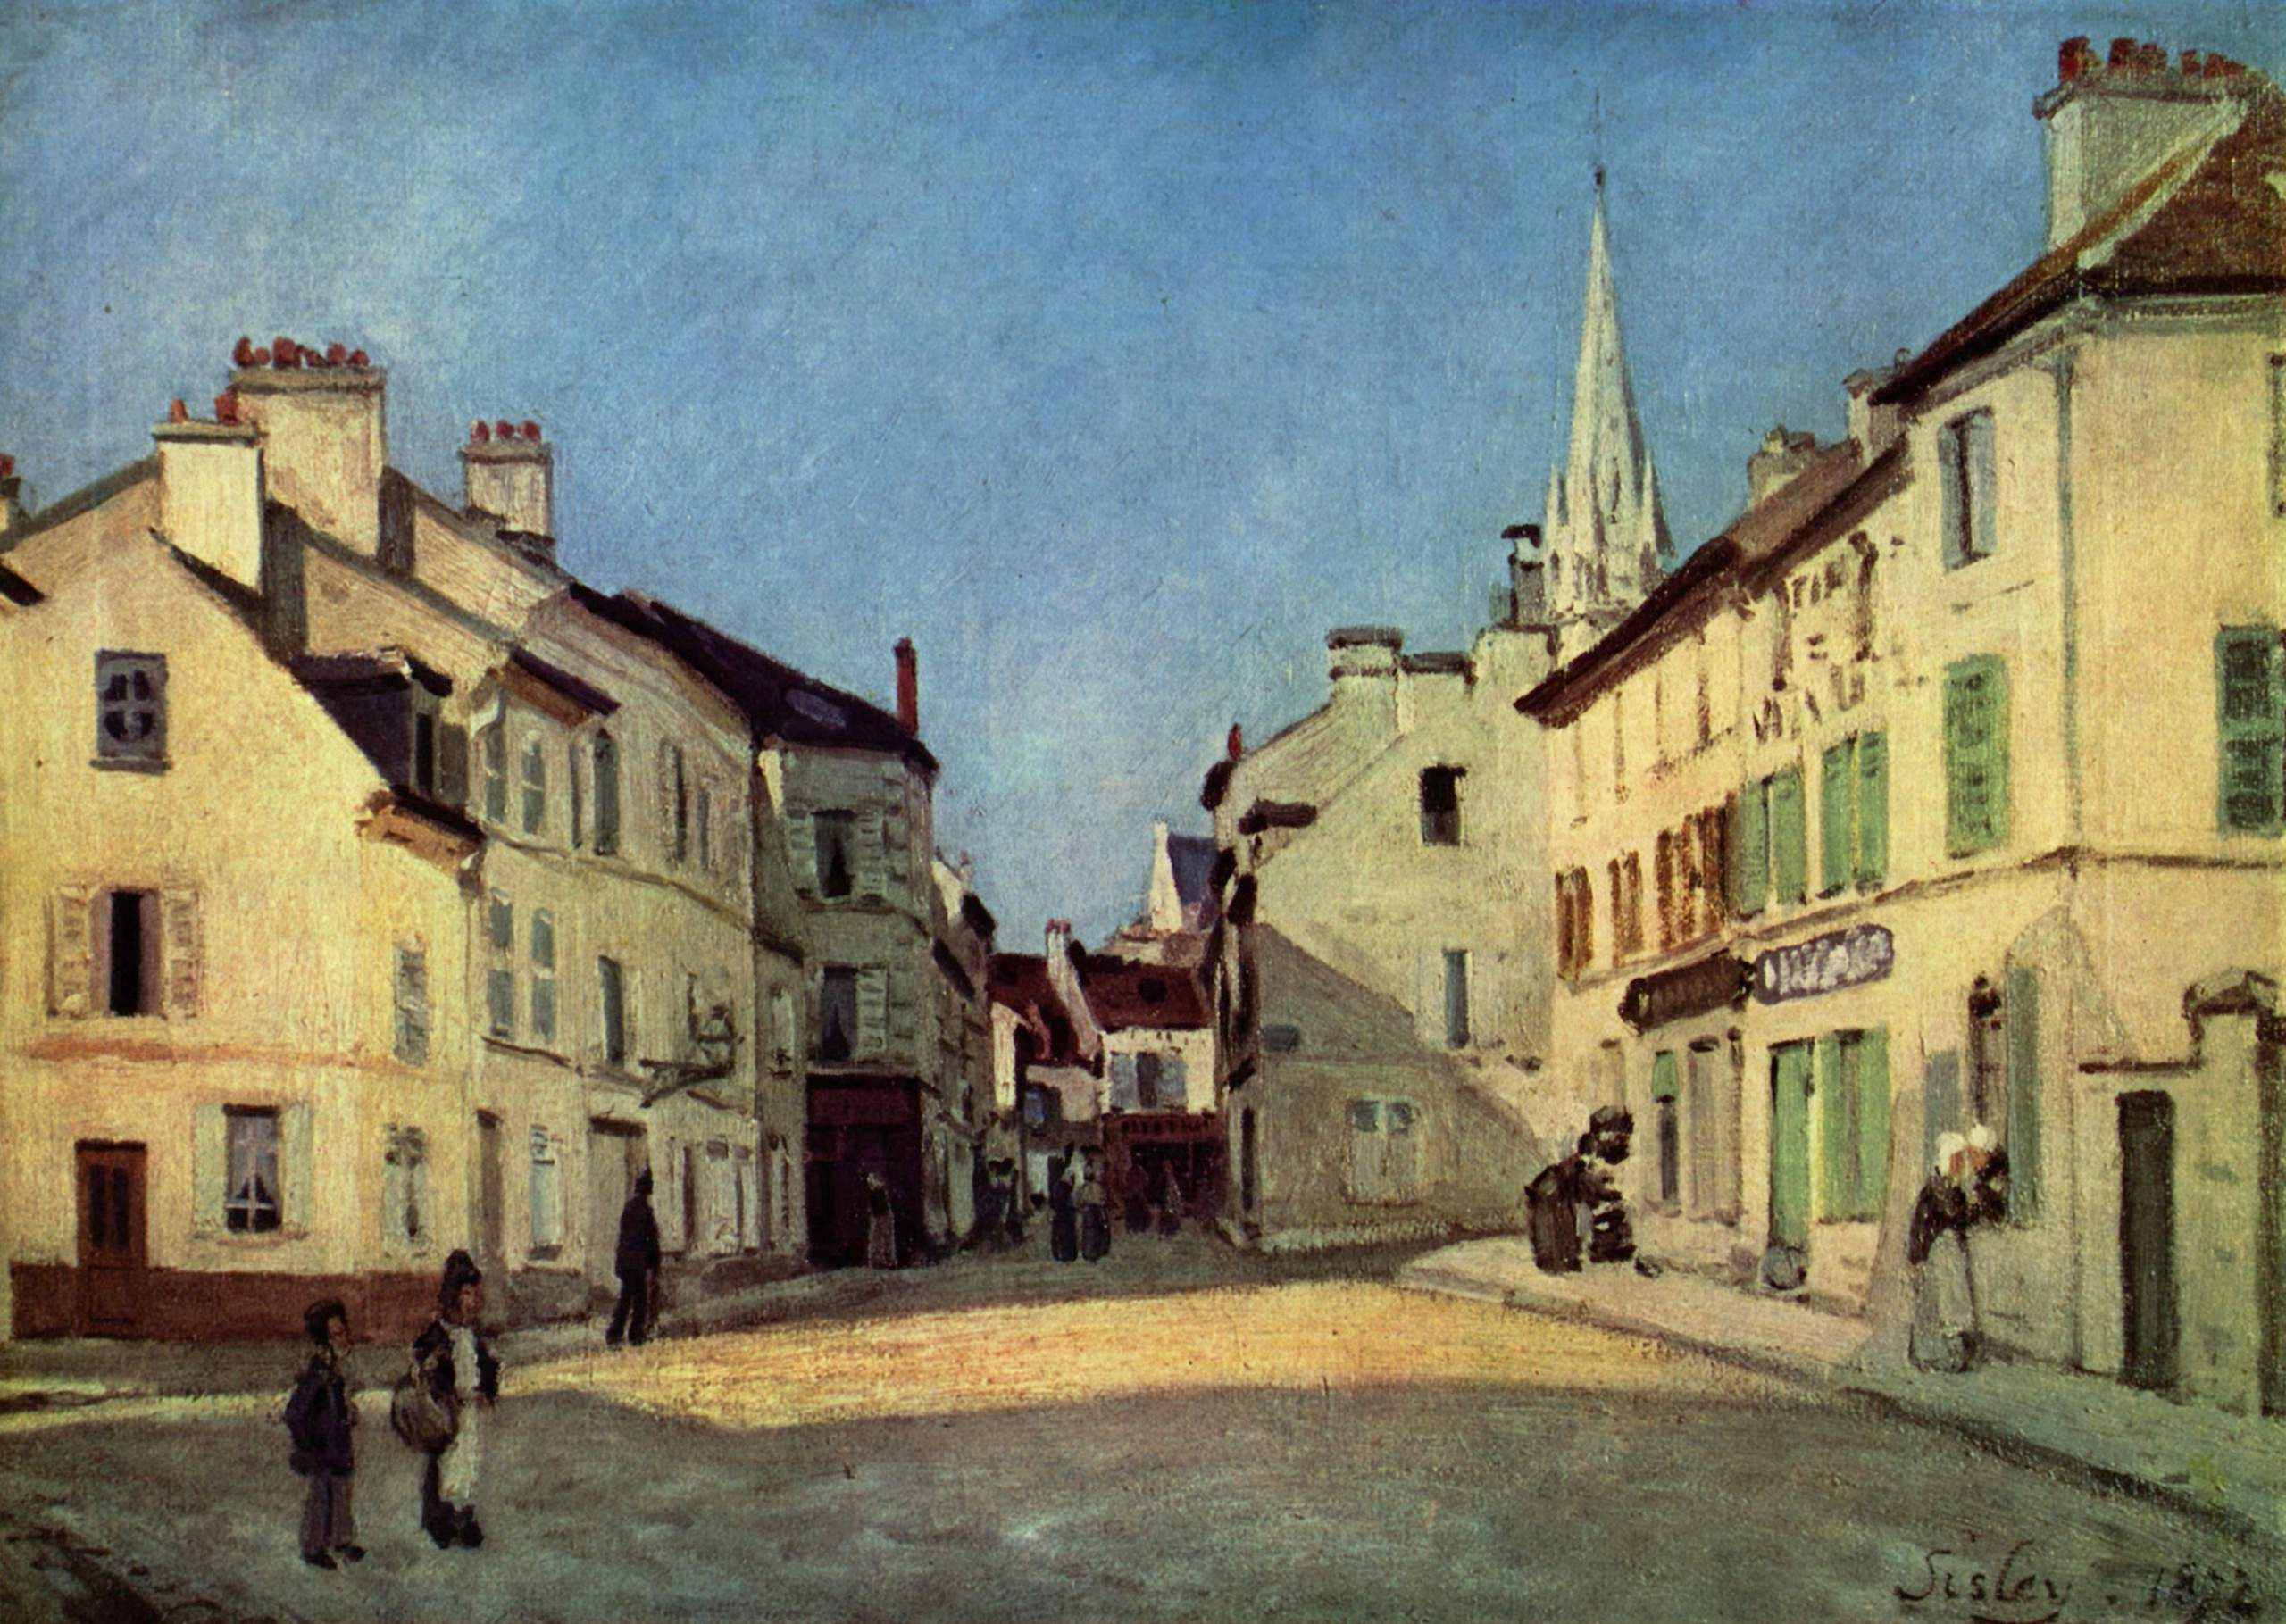
\includegraphics[width=0.7\textwidth]{Abbildungen/Bild4.jpg}
\caption{Bild 4}
\label{fig:Bild4}
\end{center}
\end{figure}

\blindtext[1]{}
\begin{table}[]
\caption{tab:Tabelle}
\begin{center}
\begin{tabular}{|c|c|}
\hline
bla & bla \\
\hline
\hline
bla & bla \\
bla & bla \\
bla & bla \\
bla & bla \\
\hline
\end{tabular}
\end{center}
\label{default}
\end{table}%

\chapter{Fazit}
\blindtext[1]{}

\blindtext[2]{}

\blindtext[2]{}

\blindtext[1]{}

\printbibliography

\end{document}  